\documentclass[conference,letterpaper]{IEEEtran}
\usepackage[T1]{fontenc}
\usepackage{amsmath,amssymb}
\usepackage{booktabs,array,graphicx}
\usepackage{cite}
\usepackage{tikz}
\usetikzlibrary{arrows.meta,positioning}
\usepackage[hidelinks]{hyperref}
\usepackage{url}
\hypersetup{
  pdftitle={Bottleneck-Guided Keccak Acceleration on an RV32 SIMT GPU},
  pdfauthor={Anonymous authors},
  pdfsubject={IEEE conference working draft, September 2026},
  pdfkeywords={ML-KEM, ML-DSA, Keccak, RV32, Vortex, SIMT, subgroup instructions}
}
\input{numbers.tex}
\makeatletter
\newcommand{\tablerows}[1]{\@@input #1 }
\makeatother
\newcommand{\code}[1]{\texttt{#1}}
\newcommand{\sg}{SG25}
\newcommand{\rot}{\operatorname{ROL}_{64}}
\newcommand{\src}[1]{\par\smallskip{\scriptsize Source: \nolinkurl{#1}.}}

\title{Bottleneck-Guided Keccak Acceleration\\on an RV32 SIMT GPU}
\author{\IEEEauthorblockN{Anonymous authors}
\IEEEauthorblockA{Working draft --- September 2026}}

\begin{document}
\maketitle
\begin{abstract}
We study bottleneck selection and instruction granularity for post-quantum
cryptography on an RV32 Vortex SIMT GPU. Software ablation attributes
\MlkKeccakShare{} of an instrumented ML-KEM-768 round trip to Keccak-f[1600]
and \MlkNttShare{} to forward and inverse number-theoretic transforms,
giving elimination bounds of \MlkKeccakBound{} and \MlkNttBound{}.
We retain C and RV32 assembly baselines, then implement THETA, RHOPI, and
CHII/IOTA as six single-destination instructions. Twenty-five lanes hold
a state in ordinary registers. A whole-round register instruction pair
and a memory-pointer permutation engine provide comparison points.
On the same 8-warp, 32-thread processor, stage instructions improve RTL
permutation throughput by \StageThroughputGain{} times over shuffle-only SG25.
With the final cooperative NTT and arithmetic path fixed, the stage backend
improves complete ML-KEM cycles by \UnifiedStageOne{} times at one request
and \UnifiedStageEight{} times at eight requests over serial software;
the instruction-only gains over the identical shuffle mapping are
\UnifiedIseOne{} and \UnifiedIseEight{} times.
At a common 250 MHz target, the stage extension adds \StageLutOverhead{} LUTs
and \StageFfOverhead{} flip-flops to the full core. Whole-round fusion raises
permutation throughput by another \RoundThroughputGain{} times, but improves
the final integrated ML-KEM by only \UnifiedRoundOne{} and
\UnifiedRoundEight{} times.
Collective granularity trades pipeline storage against benefits that
shrink substantially at application scope.
\end{abstract}
\begin{IEEEkeywords}
post-quantum cryptography, ML-KEM, ML-DSA, Keccak, RISC-V, SIMT,
instruction-set extension, FPGA
\end{IEEEkeywords}

\section{Introduction}
ML-KEM and ML-DSA standardize module-lattice mechanisms for key establishment
and digital signatures~\cite{fips203,fips204}. Their implementations combine
polynomial arithmetic with SHA-3 and SHAKE~\cite{fips202}. A processor designer
can accelerate an NTT butterfly, a Keccak stage, or an entire permutation, but
the most parallel primitive need not provide the largest application benefit.
The baseline software, the distribution of work among lanes, and the fraction
of time outside the accelerated primitive all influence the result.

An extensible GPU makes this choice particularly consequential.
Vortex supplies an open RISC-V SIMT hardware and software
stack~\cite{vortex}, allowing custom instructions to be evaluated through
software, functional simulation, processor RTL, and synthesis. A pointer
instruction can send a memory-resident Keccak state to a dedicated processing
element (PE). Alternatively, a subgroup can hold the state in ordinary lane
registers and cooperate through reductions and fixed gathers. Both may be
fast, but they exercise different parts of the GPU and impose different
integration costs.

This work asks three questions. First, how much of an unaccelerated PQC
request is actually attributable to Keccak and NTT, with a stated input and
denominator? Second, how much benefit comes from a cooperative software
mapping before adding an instruction? Third, how do stage-level and
whole-round collectives compare with a pointer PE after accounting for
complete requests and full-core implementation cost?

Our contributions are as follows.
\begin{enumerate}
\item We assemble a reproducible baseline study covering reference C,
optimized RV32 Keccak assembly, request batching, cooperative software NTT,
and component ablation. The study distinguishes measured cycle differences
from extrapolated or algebraic quantities.
\item We implement an RV32 stage-factored subgroup interface with ordinary
GPR state, explicit low/high destinations, and a full-warp execution contract.
All eight combinations of software and instruction stages are evaluated on
the same hardware.
\item We implement a whole-round GPR comparator and evaluate it alongside
the stage design and pointer PE. The comparison connects instruction
granularity to RTL throughput, ML-KEM latency, memory-operation counts,
FPGA full-core area/timing, and isolated ASIC cell area.
\end{enumerate}

We do not claim the 25-thread state layout or whole-round warp collectives
as new concepts. ML-Cube uses 25-thread Keccak with
shuffles~\cite{mlcube}, and an NVIDIA patent application describes a
64-bit warp-collective Keccak round~\cite{collectivepatent}.
Our focus is the explicit RV32 interface, its open implementation, and the
controlled comparison of granularities. The measured results do not select
one universal winner: the whole-round unit leads the GPR permutation test,
while the pointer PE leads the eight-request ML-KEM test.

\section{Background and Experimental Scope}
\subsection{PQC work and two forms of parallelism}
The measured ML-KEM-768 request includes key generation, encapsulation, and
decapsulation; the ML-DSA-65 round trip includes key generation, signing,
and verification. The software is based on mlkem-native and
mldsa-native~\cite{mlkemnative,mldsanative}. We call the number of concurrent
requests $M$. Increasing $M$ offers independent work to the warp scheduler
without shortening a particular request's dependency chain.

We use $L$ for software lanes assigned to work within a request. In the
historical x4 backend, these lanes process independent hash streams exposed
by the library API. In \sg{}, lanes cooperate on \emph{one} permutation:
lane $t=x+5y$ holds the 64-bit word $A[x,y]$, for $0\leq x,y<5$.
These mappings have different synchronization and storage requirements.
Neither their speedups nor their resource counts can be multiplied together
without an experiment that combines them.

A Keccak-f[1600] permutation consists of 24 rounds. Each round computes
column parity and the THETA correction, rotates and rearranges words in
RHOPI, then applies CHI and the IOTA round constant. This produces structured
cross-lane communication: five-word column reductions, a fixed permutation,
and three-word row gathers. The RV32 interface stores each word in two
32-bit registers, avoiding a change to the core-wide integer width.

\subsection{Measurement families and denominators}
Table~\ref{tab:config} separates the measurement families. All cycle results
are simulation results. FPGA numbers come from routed out-of-context
\code{VX\_core\_top} or isolated-unit implementations targeting the Alveo V80
part; they are not board measurements. We preserve historical software
experiments to explain the design choice, but use the 8-warp, 32-thread
experiments for the collective comparison.

\begin{table*}[t]
\caption{Experimental families. All use RV32 and one core. $W$ is resident warp
capacity, $T$ is hardware threads per warp. A request count is a separate quantity.}
\label{tab:config}
\centering\footnotesize
\begin{tabular}{@{}>{\raggedright\arraybackslash}p{.17\textwidth}p{.09\textwidth}>{\raggedright\arraybackslash}p{.20\textwidth}>{\raggedright\arraybackslash}p{.20\textwidth}>{\raggedright\arraybackslash}p{.24\textwidth}@{}}
\toprule
Family & $W\times T$ & Workload / software & Timing denominator & Scope of valid comparison \\
\midrule
Historical attribution & $4\times4$ & Single-lane ML-KEM KAT; ML-DSA fixed input & Instrumented profile's own cycles & Component ablation within that profile \\
C / assembly A/B & $4\times4$ & Same ML-KEM request; reference C or PQRV & Whole-launch device cycles & Optimized software versus C \\
Batch and x4 mapping & $8\times4$ & $M=1,2,4,8$; $L=1,2,4$ where archived & Each sweep's own $M=1,L=1$ launch & Request throughput and cache/mapping interaction \\
SG25 stages / round & $8\times32$ & 32-wide SIMD/ALU; 1 or 8 states & Synchronized permutation span & Shuffle, stage-use ablation, whole round \\
Complete SG25 ML-KEM & $8\times32$ & Serial FIPS-202; 143 permutations/request & Whole-launch cycles at fixed $M$ & SG1, shuffle, stages, whole round, pointer \\
Final NTT+Keccak ML-KEM & $8\times32$ & W32 NTT/arithmetic; KAT; 140 permutations/request & Whole-launch cycles at fixed $M$ & Five Keccak backends with all other arms fixed \\
Physical implementation & $8\times32$ & Full core, or isolated units explicitly labeled & Matched 250/300 MHz constraints & LUT/FF and STA-derived frequency \\
\bottomrule
\end{tabular}
\end{table*}

The principal collective configuration has a 32-lane ALU and LSU, 16 KiB
instruction and data caches, and 16 KiB local memory. L2/L3 are disabled.
Historical cache sweeps explicitly vary L2; their numbers are not merged
with the main configuration. SimX provides functional and timing models,
processor RTL simulation provides cycle comparisons, and XRT simulation
checks integration through the accelerator interface.

For an equal-sized batch, speedup is
\begin{equation}
S_{\mathrm{same}\ M}=\frac{C_{\mathrm{baseline}}(M)}{C_{\mathrm{candidate}}(M)}.
\end{equation}
For scaling a backend from one request to $M$, throughput gain is
\begin{equation}
G_M=\frac{M C(1)}{C(M)}.
\end{equation}
These are different denominators. Whole-launch cycles include device-side
launch setup and teardown; they exclude host transfers. Phase cycles are
intervals around the cryptographic calls. A phase total cannot silently
replace a whole-launch denominator.

\section{Software Baselines and Bottleneck Attribution}
\subsection{ML-KEM: Keccak, transforms, and the residual}
The historical ML-KEM profile uses the same FIPS 203 known-answer-test coins
as its corresponding baseline. It executes 144 scalar permutations,
including the scalar calls made through x4 fallback, and 15 forward plus
nine inverse transforms. The x4 counter records 24 wrapper calls;
\emph{it is not added as another $4\times24$ permutations} to the scalar count.

We remove either the permutation body or the forward/inverse transform
bodies through native hooks. The cryptographic outputs of these ablated
programs are intentionally invalid. They are used only to estimate component
cost, with the instrumented baseline as the denominator:
\begin{equation}
f_i=\frac{C_0-C_{-i}}{C_0},\qquad
S_{\infty,i}=\frac{C_0}{C_{-i}}=\frac{1}{1-f_i}.
\label{eq:ablation}
\end{equation}
The removed bodies retain the surrounding invocation path. The cycle
differences therefore include consequences for scheduling and memory, rather
than being a count of executed ALU operations alone.

\begin{table}[t]
\caption{ML-KEM-768 component ablation. Single lane, $4w\times4t$,
SimX; every row records 144 permutations.}
\label{tab:mlkprofile}
\centering\scriptsize\setlength{\tabcolsep}{3pt}
\begin{tabular}{@{}lrrrr@{}}
\toprule
Variant & Cycles & Removed cycles & Share & Bound \\
\midrule
\tablerows{profile_mlk.tex}
\bottomrule
\end{tabular}
\src{pqc/results/ablation_mlkem.csv}
\end{table}

Table~\ref{tab:mlkprofile} gives \MlkKeccakCycles{} removed cycles for Keccak
and \MlkNttCycles{} for NTT/INTT. Relative to \MlkProfileCycles{} profile
cycles, the shares are \MlkKeccakShare{} and \MlkNttShare{}. Thus even ideal
transform elimination yields only \MlkNttBound{}$\times$ on this workload,
whereas ideal Keccak elimination yields \MlkKeccakBound{}$\times$.
The unchanged permutation count across arms rules out a change in the
number of permutations as the explanation for the Keccak delta.
It does not establish that every data-dependent path is invariant.

Subtracting both deltas from the baseline leaves \MlkResidualCycles{}
cycles, or \MlkResidualShare{}. Figure~\ref{fig:profile} shows this
\emph{algebraic residual}. It is not a separately instrumented exclusive
category or a measured joint ablation. It can contain sampling, polynomial
operations outside NTT/INTT, packing, decoding, absorb/squeeze work, allocation,
and control. The archive does not split these contributors further, so we do
not label all residual time as memory or claim a measured combined
Keccak-plus-NTT bound.

\begin{figure}[t]
\centering\includegraphics[width=\columnwidth]{profile.pdf}
\caption{Historical component attribution from separate ablations.
Each bar has its own instrumented denominator. Hatched residuals are
obtained by subtraction; additivity has not been measured for these rows.}
\label{fig:profile}
\end{figure}

Input consistency matters because rejection sampling can change the
permutation count. The archived profile now uses KAT coins; earlier
156-permutation measurements and stale narrative percentages are excluded
from this attribution.
The main \sg{} integration instead uses fixed bytes $0,\ldots,95$ and the
library's serial FIPS-202 path, with 143 permutations in every compared
backend. We do not transfer the historical \MlkKeccakShare{} share or its
bound to that new software/configuration.

\subsection{ML-DSA: measured key generation and estimated round trips}
Table~\ref{tab:dsaprofile} gives the corresponding ML-DSA results under two
library memory budgets. Key generation admits the same ablation method:
both budgets perform 190 permutations. The Keccak deltas are 29,231,666
cycles for \code{low} and 29,119,995 for \code{full}, within 0.4\%.
The resulting elimination bounds are 3.285$\times$ and 3.912$\times$.
NTT/INTT contribute 7.13\% and 7.62\%, respectively.

\begin{table}[t]
\caption{ML-DSA-65 attribution, single lane, $4w\times4t$, SimX.
M: measured component ablations; E: extrapolated component costs.
Totals are millions of profile cycles.}
\label{tab:dsaprofile}
\centering\footnotesize\setlength{\tabcolsep}{4pt}
\begin{tabular}{@{}lrrrr@{}}
\toprule
Scope / budget & Total & Keccak & NTT/INTT & Basis \\
\midrule
\tablerows{profile_dsa.tex}
\bottomrule
\end{tabular}
\src{pqc/results/ablation_mldsa.csv}
\end{table}

Signing and verification do not admit this substitution.
Stubbing the hash during signing changes the rejection loop; stubbing it
during verification can make \code{SampleInBall} fail to terminate normally.
The round-trip entries therefore multiply call counts by component costs
calibrated from key generation. They are estimates, not direct
measurements of signing/verification time in each primitive.
For the archived input, the low/full round trips execute 782/582
permutations and 103/95 transforms. Their estimated Keccak shares are
63.34\%/62.76\%; transform shares are 14.78\%/18.12\%.
The memory budget changes the workload composition as well as its total.

These ML-DSA round-trip values describe one input's rejection-loop outcome.
An earlier host distribution was not completely archived and had an
overflowing histogram; its tail statistics are not used here.
A separate, correct pointer-PE experiment reaches 2.652$\times$/2.628$\times$
round-trip speedups for low/full budgets, supporting the scale of the
hash-cost estimate without supplying a missing input distribution.

\subsection{An optimized software baseline}
Reference C alone is insufficient to evaluate an instruction extension.
We therefore also use PQRV's hand-written RV32 Keccak implementation,
introduced through the library's native permutation hook~\cite{pqrv}.
Table~\ref{tab:software} compares these columns in one historical
$4w\times4t$ experiment. The NTT implementation is unchanged by the swap.

\begin{table}[t]
\caption{Reference C versus PQRV assembly on the same historical
single-lane ML-KEM configuration. Ratio is C/assembly.}
\label{tab:software}
\centering\footnotesize\setlength{\tabcolsep}{4pt}
\begin{tabular}{@{}lrrr@{}}
\toprule
Metric & Reference C & RV32 assembly & Ratio \\
\midrule
\tablerows{software.tex}
\bottomrule
\end{tabular}
\src{pqc/results/keccak_baseline_columns.csv}
\end{table}

Assembly improves the permutation by 1.131$\times$ and the complete launch
by 1.080$\times$. Using the profile share in
$1/(1-f_K+f_K/s_K)$ predicts approximately 1.082$\times$,
a cross-check rather than a replacement for the measured launch.
In a separately archived, internally matched three-arm run, reference C,
assembly, and the pointer PE take 32,778,558, 30,321,833, and 11,527,027
cycles. That run gives a 2.844$\times$ PE gain over C and 2.631$\times$
over assembly. These counts come from \code{keccak\_ise\_simx.csv};
they must not be divided into the totals in Table~\ref{tab:software}.

\subsection{Cooperative NTT as a control}
The cooperative forward NTT maps each layer's 128 butterflies across $L$
lanes. It uses the library's arithmetic and twiddle factors and a shared
polynomial array, with visibility fences between layers.
Every result is checked coefficient by coefficient against the library.
Table~\ref{tab:ntt} reports both the optimized library denominator and the
cooperative implementation's own one-lane denominator.

\begin{table}[t]
\caption{Software forward NTT for ML-KEM. The library reference takes
133,526 cycles. Mismatch count is zero in all rows.}
\label{tab:ntt}
\centering\footnotesize\setlength{\tabcolsep}{4pt}
\begin{tabular}{@{}rrrr@{}}
\toprule
$L$ & Cooperative cycles & Gain vs library & Gain vs coop. $L=1$ \\
\midrule
\tablerows{ntt.tex}
\bottomrule
\end{tabular}
\src{pqc/results/ntt_cooperative.csv}
\end{table}

Four lanes deliver 3.940$\times$ scaling of the cooperative code, but only
2.487$\times$ over the faster single-lane library. Indexing and fences
make the cooperative one-lane arm slower. This distinction prevents a
3.940$\times$ scaling result from being presented as the benefit over
existing software. The experiment covers a forward transform, not an
integrated NTT/INTT extension or complete-KEM speedup.

Microbenchmark setup is another source of bias. The original forward-NTT
microbenchmark times coefficient reconstruction with the transform, reporting
160,270.4 cycles rather than the 133,526-cycle transform-only reference.
Multiplying such a setup-inclusive cost by application call counts would
overstate the transform share. We use application ablation for attribution
and transform-only timing for this software control.

\subsection{Request batching, lane width, and memory budget}
Table~\ref{tab:batch} shows that scheduling independent requests recovers
throughput without an instruction extension. ML-KEM reaches
6.654$\times$ at eight requests on an eight-warp, four-thread core.
ML-DSA has archived points through four requests in this baseline family.
The table reports $M C(1)/C(M)$, not reduced latency of one request.

\begin{table}[t]
\caption{Unmodified-software request batching, $8w\times4t$, one active
lane per request, L2/L3 off. Cycles are millions per complete batch.}
\label{tab:batch}
\centering\footnotesize
\begin{tabular}{@{}lrrr@{}}
\toprule
Scheme & $M$ & Batch cycles & Throughput gain \\
\midrule
\tablerows{batch.tex}
\bottomrule
\end{tabular}
\src{pqc/results/batch_baseline.csv}
\end{table}

Increasing request concurrency and within-request lane width together can
be counterproductive. Figure~\ref{fig:grid} preserves an independent
historical ML-KEM x4 sweep with 156 scalar-equivalent permutations for its
one-lane arm. At $M=8$, L2 off, increasing $L$ from one to four changes the
throughput gain from 6.739 to 4.016. With L2 on, the corresponding values
are 7.145 and 8.280. This is evidence for a cache-sensitive interaction
between mappings, not a universal benefit of wider launches.

\begin{figure}[t]
\centering\includegraphics[width=\columnwidth]{batch_width.pdf}
\caption{Historical ML-KEM x4 mapping sweep on $8w\times4t$.
Both panels use the sweep's L2-off, $M=1,L=1$ baseline of 36,614,668 cycles.
Source: \texttt{mlkem\_MxL.csv}. These inputs/backend differ from the
KAT ablation and the serial-FIPS-202 SG25 experiment.}
\label{fig:grid}
\end{figure}

ML-DSA adds another software choice. Table~\ref{tab:ram} varies library
memory budget and x4 lane width for one request.
The full-budget implementation uses an 86,912-byte arena rather than
21,568 bytes. With the low budget, four lanes provide no gain; with the
full budget they improve launch time by 1.601$\times$ over that budget's
one-lane arm. Changing both budget and mapping produces 2.118$\times$
over low-budget, one-lane software, without new hardware.

\begin{table}[t]
\caption{ML-DSA software memory-budget/width control, $8w\times4t$,
one request, L2/L3 off. Gain is relative to low-budget $L=1$.}
\label{tab:ram}
\centering\footnotesize
\begin{tabular}{@{}lrrrr@{}}
\toprule
Budget & $L$ & Mcycles & Arena bytes & Gain \\
\midrule
\tablerows{ram.tex}
\bottomrule
\end{tabular}
\src{pqc/results/mldsa_ram_x_lane.csv}
\end{table}

\section{An RV32 Subgroup Keccak Interface}
\subsection{State placement and programming contract}
One 32-thread warp holds one state. Lanes 0--24 each hold a 64-bit word as
two ordinary 32-bit GPR values. Lanes 25--31 carry no state and return zero.
All 32 lanes must execute each collective with the full mask at the same
instruction. In particular, guarding the collective with
\code{lane < 25} violates the contract. Guarded loads/stores are allowed
if the warp reconverges before the collective.

Each instruction snapshots its complete source vectors and writes one
destination vector. It has no pointer operand, memory ordering effect,
hidden round counter, or private architectural state. Ordinary RAW hazards,
backpressure, and writeback arbitration still apply. Transient pipeline
registers are microarchitectural storage and are included in the area cost.

The initial implementation requires RV32, 32 threads, a 32-wide SIMD
datapath, and 32 ALU lanes. A narrower packetized ALU would need operand
collection across packets; warp width alone is insufficient.
The 25-of-32 state layout uses 78.125\% of lanes for state words. The
remaining lanes still consume execution resources. We do not assume that
this utilization loss is free.

\subsection{Three stages, six single-destination instructions}
For $t=x+5y$, let $A[x,y]$ combine the low/high inputs.
All coordinates wrap modulo five. THETA computes
\begin{align}
C[x]&=\bigoplus_{y=0}^{4} A[x,y],\\
T[x,y]&=A[x,y]\oplus C[x-1]\oplus\rot(C[x+1],1).
\end{align}
\code{KTHETA.L/H.SG25} each read both state halves and select one output
half. Cross-half carry bits from the one-bit rotation are part of the
operation; two independent 32-bit reductions would be incorrect.

RHOPI combines a fixed rotation with the lane permutation:
\begin{equation}
B[y,(2x+3y)\bmod5]=\rot(T[x,y],r[x,y]).
\end{equation}
At destination $(x_d,y_d)$, the source is
$x_s=(x_d+3y_d)\bmod5,\ y_s=x_d$.
\code{KRHOPI.L/H.SG25} select the corresponding result half. Rotation
amounts belong to source coordinates, which is essential when implementing
the inverse gather.

CHII evaluates each 32-bit half independently:
\begin{equation}
U[x,y]=B[x,y]\oplus(\neg B[x+1,y]\land B[x+2,y]).
\end{equation}
Only lane zero then XORs its half of $RC[q]$. Unlike THETA/RHOPI,
\code{KCHII.L/H.SG25} read one state half and a uniform round index $q$,
not both state halves. All lanes, including padding lanes, must supply the
same index in $0,\ldots,23$.

The six encodings use CUSTOM0 (\code{0x0b}), \code{funct7=0x06},
with \code{funct3=0..5}. The extension uses two source-vector reads and
one destination-vector write per instruction.
THETA and RHOPI low/high operations must read the same old state:
\begin{equation}
(a_l,a_h)\rightarrow(t_l,t_h)\rightarrow(b_l,b_h)
\rightarrow(a'_l,a'_h).
\end{equation}
Overwriting $a_l$ before the high THETA operation would break this
dependency. Two GPRs describe persistent state capacity, not peak register
pressure. The all-stage permutation loop uses five GPRs for state,
temporaries, round, and loop limit; its disassembly has no load, store,
call, or stack frame.

\subsection{ALU integration and the whole-round comparator}
Figure~\ref{fig:architecture} contrasts the architectural boundaries.
The stage unit sits under \code{VX\_alu\_unit} and uses two registered
pipeline stages. THETA forms parity then the correction; RHOPI and CHII
use the same latency interface. The direct unit latency is two cycles
with initiation interval one. These values are not the core's observed
dependent instruction latency.

The source code expresses the fixed cross-lane connections directly.
It shares the core's operand and result interfaces, but the current
implementation does \emph{not} establish physical sharing of the existing
general shuffle network. A claim of shuffle-network area reuse would
require a different integration and its own synthesis evidence.

\begin{figure*}[t]
\centering
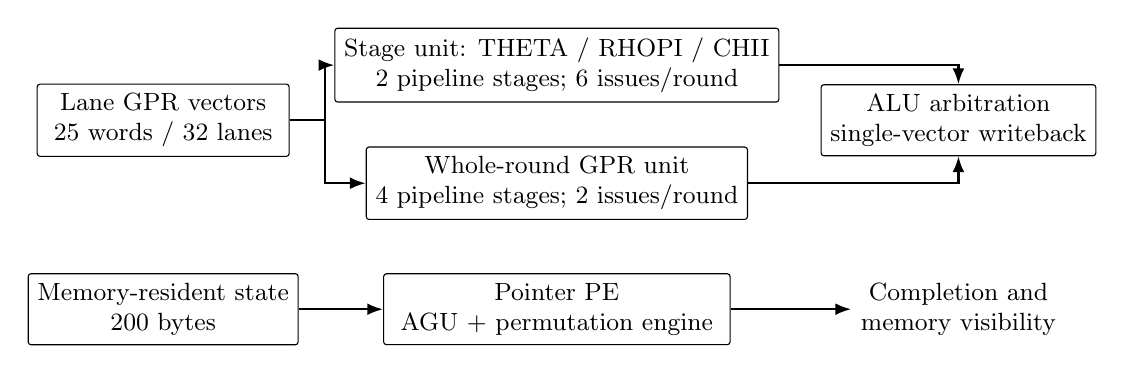
\begin{tikzpicture}[
  box/.style={draw,rounded corners=1pt,align=center,minimum height=9mm,font=\small},
  arr/.style={-{Latex[length=2mm]},thick}]
\node[box,minimum width=32mm] (regs) at (0,0) {Lane GPR vectors\\25 words / 32 lanes};
\node[box,minimum width=44mm] (stage) at (5.0,0.7) {Stage unit: THETA / RHOPI / CHII\\2 pipeline stages; 6 issues/round};
\node[box,minimum width=44mm] (round) at (5.0,-0.8) {Whole-round GPR unit\\4 pipeline stages; 2 issues/round};
\node[box,minimum width=26mm] (wb) at (10.1,0) {ALU arbitration\\single-vector writeback};
\draw[arr] (regs.east) -- ++(.45,0) |- (stage.west);
\draw[arr] (regs.east) -- ++(.45,0) |- (round.west);
\draw[arr] (stage.east) -| (wb.north);
\draw[arr] (round.east) -| (wb.south);
\node[box,minimum width=32mm] (mem) at (0,-2.4) {Memory-resident state\\200 bytes};
\node[box,minimum width=44mm] (ptr) at (5.0,-2.4) {Pointer PE\\AGU + permutation engine};
\node[align=center,font=\small] (done) at (10.1,-2.4) {Completion and\\memory visibility};
\draw[arr] (mem.east) -- (ptr.west);
\draw[arr] (ptr.east) -- (done.west);
\end{tikzpicture}
\caption{Alternative Keccak execution boundaries. GPR stages and the whole-round
unit use ordinary ALU operand/writeback interfaces. The pointer PE transfers a
memory-resident state. Pipeline storage is charged to each implementation.}
\label{fig:architecture}
\end{figure*}

The independent whole-round extension uses CUSTOM2 (\code{0x5b}).
\code{funct3=0/1} selects \code{KROUND.L/H.SG25}; \code{funct7} carries
a literal round index. Both source vectors contain the old low/high state,
and each issue computes one selected half of a complete round.
The four registered stages are column parity, THETA, RHOPI, and CHII/IOTA.
Direct latency is four cycles and initiation interval is one.
There is no hidden state retained between issued instructions.
The low/high pair recomputes from the same old state; it is not a
dual-writeback macro-operation.

Literal round encoding expands 24 rounds into 48 instructions. The
stage kernel retains a round loop with six collectives, an increment,
and a branch per round. Consequently, the measured comparison includes
both the instruction granularity and its present code generation.
It is not an isolated comparison with identical loop-control instructions.

The pointer \code{KECCAKF} baseline remains a full-permutation engine
connected through the existing SFU/memory path. It supplies a useful
dedicated-engine reference, whereas the GPR variants expose lane-vector
data directly to the execution unit. The pointer design requires
architectural state transfer through the memory interface for each invocation.

\subsection{Full SHAKE and ML-KEM mapping}
The subgroup sponge retains state in lane registers across absorb,
permutation, and squeeze within a one-shot call. Absorb uses ordinary
loads/XORs; squeeze uses ordinary stores. Incremental SHAKE128 saves a
word per lane in its context across separate API calls and reloads it
on reentry. Thus register residence within a call does not mean the
incremental context never touches memory.

For ML-KEM, lane zero executes the surrounding serial library. A
\code{TMC} boundary and a noinline worker activate the complete warp
for FIPS-202, broadcast arguments, run the subgroup sponge, and restore
the leader mask on return. A shared allocation arena avoids allocating
the same request's workspace 32 times.

A correctness-first alternative ran the outer KEM redundantly on every
lane. We preserve its results as a control. It satisfies output checks
but causes excessive memory operations and contention.
Removing that redundancy is a software mapping improvement and must
not be attributed solely to the Keccak instructions.

\section{Evaluation}
\subsection{Correctness and timing methodology}
Stage tests cover aliases, zero registers, high/low bit crossings, padding
lanes, all round constants, metadata, and backpressure. The mixed stage
RTL unit test has 288 transactions; the whole-round test has 192.
Contract tests diagnose partial masks and invalid rounds, plus nonuniform
round operands for CHII. These checks diagnose unsupported programming
conditions; they do not define a production trap ABI.

Full-round checks use 17 states and 10,200 word comparisons. Complete
SHAKE128/256 tests cover 204 input/output cases, including empty messages,
unaligned addresses, and rate boundaries. SimX and XRT integration tests
pass. ML-KEM checks return codes, shared-secret agreement, and checksums
of the public key, secret key, ciphertext, and shared secret.

Permutation timing launches one state per warp and brackets a dependent
chain with synchronized cycle reads. CTA barriers keep initial state loads
and final stores outside the timed batch; the measured span is
$\max(t_{\mathrm{end}})-\min(t_{\mathrm{start}})$.
It includes scheduling skew and any accesses performed inside software
stages. For the eight-arm stage study, the marginal cost is
\begin{equation}
c_{\mathrm{marginal}}=
\frac{\operatorname{span}(8)-\operatorname{span}(4)}{4M}.
\label{eq:marginal}
\end{equation}
The whole-round comparison uses a separate 64-permutation chain and
reports $\operatorname{span}(64)/(64M)$. These estimators are kept
separate in the tables.

Across the 32 matched points in the stage dataset, retired instruction
counts agree between SimX and processor RTL; maximum whole-launch cycle
difference is \StageMaxModelGap{}. Passing this set establishes agreement
on the tested cases, not a complete proof of the timing model.
The complete ML-KEM XRT checks are integration/correctness results;
the internally matched SimX rows supply the application comparisons.

\subsection{Eight-way instruction-use ablation}
Table~\ref{tab:stages} uses one hardware build with all six stage encodings
enabled. Each arm replaces selected shuffle-software stages with custom
instructions. Therefore it measures instruction use, not the physical
area obtained by synthesizing only one selected stage.

\begin{table}[t]
\caption{RTL marginal permutation cost from Eq.~\ref{eq:marginal}.
T/R/C indicate THETA, RHOPI, CHII instructions.
Gains use the shuffle-only \texttt{---} arm at the same batch size.}
\label{tab:stages}
\centering\footnotesize\setlength{\tabcolsep}{4pt}
\begin{tabular}{@{}lrrrr@{}}
\toprule
Arm & 1-state cyc. & Gain & 8-warp cyc./perm. & Gain \\
\midrule
\tablerows{stages.tex}
\bottomrule
\end{tabular}
\src{pqc/results/keccak_sg25_stages.csv}
\end{table}

The complete stage design reduces dependent marginal cost from 19,285.75
to 2,050 cycles, a \StageLatencyGain{}$\times$ gain. Eight-warp cost falls
from 6,215.59 to 481.50 cycles per completed permutation,
a \StageThroughputGain{}$\times$ gain. Figure~\ref{fig:stages} shows that
stage benefits depend on the load point: RHOPI gives the largest
single-stage latency improvement, while THETA gives the largest
single-stage eight-warp improvement. Combined benefits are not obtained
by adding the individual speedups.

\begin{figure}[t]
\centering\includegraphics[width=\columnwidth]{stage_gains.pdf}
\caption{Stage instruction-use gains on the same $8w\times32t$ hardware.
The latency and throughput denominators differ as defined in
Table~\ref{tab:stages}.}
\label{fig:stages}
\end{figure}

\subsection{Whole-round fusion}
Table~\ref{tab:rounds} gives the longer-chain comparison. The whole-round
unit improves RTL single-state cost from 2,052.219 to 499.266 cycles and
eight-warp cost from 481.664 to 117.693 cycles per completed permutation.
This is 4.110$\times$ latency improvement and
\RoundThroughputGain{}$\times$ throughput improvement.

\begin{table}[t]
\caption{64-permutation GPR chains on $8w\times32t$.
Costs are span/(64$M$), excluding initial/final state I/O.}
\label{tab:rounds}
\centering\footnotesize\setlength{\tabcolsep}{4pt}
\begin{tabular}{@{}llrr@{}}
\toprule
Model & Unit & 1-state cycles & 8-warp cyc./perm. \\
\midrule
\tablerows{rounds.tex}
\bottomrule
\end{tabular}
\src{pqc/results/keccak_kround25.csv}
\end{table}

The result makes whole-round fusion a strong implemented comparator.
The reduction from six to two issues is not, by itself, a prediction of
these cycle ratios. Loop control, register dependencies, issue arbitration,
and pipeline timing contribute to the measured sequence.

\subsection{Complete ML-KEM}
Table~\ref{tab:kem} compares complete launches on the same core geometry,
cache configuration, fixed coins, and serial FIPS-202 path.
All arms perform 143 permutations per request. SG1 and shuffle controls
run with the stage extension present but unused. The whole-round arm
enables its independent extension; the pointer arm enables PQC and KSG25.
These enable sets are recorded in the source data.

\begin{table}[t]
\caption{Complete ML-KEM-768 on SimX, $8w\times32t$.
Cycles are millions per launch; gains use SG1 at the same $M$.}
\label{tab:kem}
\centering\footnotesize\setlength{\tabcolsep}{3pt}
\begin{tabular}{@{}lrrrr@{}}
\toprule
Backend & $M=1$ & Gain & $M=8$ & Gain \\
\midrule
\tablerows{kem.tex}
\bottomrule
\end{tabular}
\src{pqc/results/keccak_sg25_mlkem.csv}
\end{table}

The shuffle-only cooperative mapping already improves launch cycles by
\KemMappingOne{}$\times$ at one request and \KemMappingEight{}$\times$
at eight requests. Replacing its permutation stages with instructions
adds \KemIseOne{}$\times$ and \KemIseEight{}$\times$, yielding total
gains of \KemStageOne{}$\times$ and \KemStageEight{}$\times$ over SG1.
This matched shuffle denominator isolates the instruction contribution
from the substantial benefit of mapping state across registers.

\begin{figure}[t]
\centering\includegraphics[width=\columnwidth]{kem_gains.pdf}
\caption{Complete-launch gains over SG1 at equal request count. The
whole-round unit's large permutation advantage produces a small additional
application gain. The pointer PE leads the eight-request launch.}
\label{fig:kem}
\end{figure}

Whole-round fusion adds only \KemRoundOne{}$\times$ and
\KemRoundEight{}$\times$ over the stage backend, despite the roughly
fourfold isolated permutation improvement. The single-request instruction
count falls from 1,093,915 to 1,073,037, just 1.91\%.
The evidence identifies a limit to further permutation optimization.
It does not yet quantitatively partition the remainder among
absorb/extract, wrappers, transforms, other polynomial work, and allocation.

The stage backend is 1.058$\times$ faster than the pointer PE for one request.
At eight requests the pointer PE is 1.130$\times$ faster than stages and
1.116$\times$ faster than the whole-round backend.
These results are compatible: a dedicated engine can benefit a saturated
request stream even when a register-resident mapping has lower latency
for a single request.

\subsection{Phase costs and memory-operation evidence}
Table~\ref{tab:phases} makes the single-request phase totals explicit.
The final column is launch cycles minus the sum of three measured call
intervals; it is not an attributed cryptographic primitive.
For SG1, key generation, encapsulation, decapsulation, and this remainder
account for approximately 28.36\%, 31.82\%, 38.39\%, and 1.43\%
of the launch. For stages they account for 23.74\%, 32.60\%, 39.56\%,
and 4.10\%. These phase shares are independent of the historical
Keccak/NTT component shares.

\begin{table}[t]
\caption{Single-request ML-KEM phase intervals, millions of cycles.
Remainder = whole launch minus phase sum.}
\label{tab:phases}
\centering\footnotesize\setlength{\tabcolsep}{3pt}
\begin{tabular}{@{}lrrrr@{}}
\toprule
Backend & KeyGen & Encaps & Decaps & Remainder \\
\midrule
\tablerows{phases.tex}
\bottomrule
\end{tabular}
\end{table}

Table~\ref{tab:traffic} reports whole-launch LSU operation counters and
the stack watermark for one request. These counts are neither transferred
bytes nor off-chip traffic, and they do not isolate register spills.
The stage and whole-round arms have identical load/store counts;
fusion primarily changes the permutation instruction sequence.
The stage permutation loop itself contains no memory instructions,
whereas the surrounding sponge and KEM still access memory.

\begin{table}[t]
\caption{Single-request whole-launch memory-operation counts and stack
watermarks. All backends use a 19,232-byte peak allocation arena.}
\label{tab:traffic}
\centering\footnotesize\setlength{\tabcolsep}{4pt}
\begin{tabular}{@{}lrrr@{}}
\toprule
Backend & Loads & Stores & Stack bytes \\
\midrule
\tablerows{traffic.tex}
\bottomrule
\end{tabular}
\end{table}

The redundant outer-KEM control incurs 7,924,185 load/store operations,
versus 326,504 for the stage leader mapping, approximately 24.3 times
as many. At eight requests the redundant version takes 160.039 million
cycles, slower than serial SG1. Correct output and a low instruction count
alone therefore do not establish an efficient SIMT mapping.

\subsection{Final NTT--Keccak integration}
Table~\ref{tab:unifiedkem} repeats the five-backend comparison after fixing
the final W32 NTT and cooperative arithmetic configuration. Every arm uses
the same combined hardware build, serial FIPS-202 call graph, and FIPS 203
KAT coins. Each request executes 140 Keccak-f permutations, 15 forward NTTs,
and nine inverse NTTs; all public keys, secret keys, ciphertexts, and shared
secrets match byte-for-byte. Consequently, only the Keccak backend varies.

\begin{table}[!h]
\caption{Final integrated ML-KEM-768 on SimX, $8w\times32t$.
Cycles are millions per launch; gains use SG1 at the same $M$.}
\label{tab:unifiedkem}
\centering\footnotesize\setlength{\tabcolsep}{3pt}
\begin{tabular}{@{}lrrrr@{}}
\toprule
Backend & $M=1$ & Gain & $M=8$ & Gain \\
\midrule
\tablerows{unified_kem.tex}
\bottomrule
\end{tabular}
\src{pqc/results/keccak_ntt_unified_mlkem.csv}
\end{table}

Stages achieve \UnifiedStageOne{}$\times$/\UnifiedStageEight{}$\times$
over SG1 at $M=1/8$. Relative to the matched shuffle implementation, the
instruction-only gains are \UnifiedIseOne{}$\times$/\UnifiedIseEight{}$\times$.
Whole-round fusion adds \UnifiedRoundOne{}$\times$/\UnifiedRoundEight{}$\times$
over stages. The latency--throughput crossover remains: stages and the
whole-round unit beat the pointer PE at $M=1$ by
\UnifiedStageVsPointerOne{}$\times$ and \UnifiedRoundVsPointerOne{}$\times$,
whereas the pointer PE leads them at $M=8$ by
\UnifiedPointerVsStageEight{}$\times$ and \UnifiedPointerVsRoundEight{}$\times$.

Full XRT integration runs for stages and whole round reproduce the KAT and
retired-instruction counts. Their whole-launch cycle gaps from SimX are
\UnifiedXrtGapStage{} and \UnifiedXrtGapRound{}, respectively. These runs
cover the AFU and processor RTL. Since all three accelerators are instantiated
in the common core, Table~\ref{tab:unifiedkem} is a functional and cycle
comparison; per-backend area still comes from the separate builds in
Section~VI.

\section{Implementation Cost}
\subsection{Full-core FPGA area and timing}
We target \code{xcv80-lsva4737-2MHP-e-S} with Vivado 2025.1,
using post-route physical optimization.
Table~\ref{tab:coreppa} compares each extension with the base core
under the same target constraint. At 250 MHz, the stage core adds 2,216 LUTs
and 1,899 FFs, or \StageLutOverhead{} and \StageFfOverhead{}.
The whole-round core adds 2,760 LUTs and 6,255 FFs. The pointer core adds
11,845 LUTs; its full-core FF count is absent from the archived row.

\begin{table}[t]
\caption{Full-core V80 routed results. Target and STA-derived $f_{\max}$
are MHz; WNS is ns. A dash is an unrecorded value, not zero.}
\label{tab:coreppa}
\centering\scriptsize\setlength{\tabcolsep}{3.5pt}
\begin{tabular}{@{}rlrrrr@{}}
\toprule
Target & Core & LUT & FF & WNS & $f_{\max}$ \\
\midrule
\tablerows{core_ppa.tex}
\bottomrule
\end{tabular}
\src{pqc/results/keccak_sg25_ppa.csv}
\end{table}

The 300 MHz implementations all have negative slack, so they do not
close that target. The whole-round build reaches an STA-derived
294.9 MHz, compared with 291.6 MHz for stages and 294.2 MHz for the base.
These are $1000/(P-\mathrm{WNS})$ estimates from the routed design,
not measured operating clocks or proof of a separate run at that estimate.
At 250 MHz all reported cores meet setup timing, with zero margin
for the whole-round and pointer cases.

The whole-round hierarchy contributes 2,483 LUT/6,130 FF at 250 MHz and
2,428 LUT/6,131 FF at the 300 MHz target. Its 300 MHz worst path is in the
local-memory response crossbar; none of the 100 reported worst paths
enters that unit. This supports timing viability of the added datapath
in this implementation, without implying it cannot affect placement
elsewhere. Small ordering differences among the Fmax estimates are not
treated as a general architectural frequency advantage.

The wide core itself must also be charged. The historical 300 MHz base
configuration grid uses 42,553 LUTs at $8w\times4t$, 148,827 at
$8w\times16t$, and 325,407 at $8w\times32t$.
Consequently, a sub-1\% extension overhead relative to the chosen wide
core is not a sub-1\% cost of widening a narrow GPU. The SG25 study fixes
the wide core to isolate instruction granularity.

\subsection{Isolated-unit FPGA and ASIC comparisons}
Tables~\ref{tab:unitfpga} and~\ref{tab:unitasic} compare isolated units.
The pointer unit performs a complete permutation, stages execute one
selected RV32 stage instruction, and the whole-round unit executes one
selected half of a round. Unit area is therefore not a same-operation
latency comparison.

\begin{table}[t]
\caption{Isolated units on V80, 300 MHz target.}
\label{tab:unitfpga}
\centering\footnotesize
\begin{tabular}{@{}lrrr@{}}
\toprule
Unit & LUT & FF & STA $f_{\max}$ (MHz) \\
\midrule
\tablerows{fpga_unit.tex}
\bottomrule
\end{tabular}
\end{table}

\begin{table}[t]
\caption{Isolated ASAP7 RVT, TT, 1.00 V, 25$^\circ$C.
Yosys 0.57 / OpenSTA 2.7.0; matched 500 MHz mapping constraint.
Area is $\mu\mathrm{m}^2$; these are mapped, not routed, ASIC results.}
\label{tab:unitasic}
\centering\footnotesize\setlength{\tabcolsep}{4pt}
\begin{tabular}{@{}lrrr@{}}
\toprule
Unit & Total area & Sequential area & STA MHz \\
\midrule
\tablerows{asic_unit.tex}
\bottomrule
\end{tabular}
\end{table}

The whole-round unit uses 7.48\% fewer isolated FPGA LUTs than stages,
but 2.990 times the FFs. On the predictive ASAP7 library~\cite{asap7},
it uses 2.123 times the total cell area and 2.989 times the sequential
area. Its larger register footprint is visible after full-core FPGA
integration, but LUT-only normalization largely hides it.

At common 250 MHz, the 64-chain RTL results and full-core LUT counts give
a whole-round versus stage throughput/LUT ratio of
\begin{equation}
\frac{481.664}{117.693}\times\frac{325{,}288}{325{,}832}
\simeq \RoundLutEfficiency{}.
\end{equation}
Thus the whole-round unit also wins this FPGA efficiency metric for pure
permutation. It would be misleading to claim that the stage design wins
all area-normalized metrics because it has fewer pipeline registers.
Conversely, dividing the same pure-permutation gain by isolated ASIC area
does not yield a measured full-ASIC application efficiency.
We omit power/energy claims because no workload-activity-based power
measurement is available.

\section{Related Work and Interpretation}
PQRV optimizes Keccak and polynomial arithmetic for several RISC-V ISA
variants~\cite{pqrv}. It motivates an assembly baseline rather than reliance
on portable C alone. Bolat et al.\ study a custom SHA-3 instruction and
its pipeline/storage integration in a RISC-V CPU~\cite{bolat}.
These approaches show that instruction acceleration and baseline selection
already have substantial prior work; the extra question here is how
cooperating SIMT lane registers change the design boundary.

ML-Cube combines register-oriented polynomial computation with GPU
execution and describes a 25-thread shuffle mapping for Keccak in
Sec.~5.1.1~\cite{mlcube}. We use this mapping as prior art and as a
software denominator. We do not compare its commercial-GPU timing
numerically against a single FPGA soft core.

Listing~3 of NVIDIA's published application describes
\code{keccak1.sync.aligned.u64}, where lanes 0--24 hold 64-bit
input/output words and a warp-collective invocation performs one
round~\cite{collectivepatent}. The text also discusses multiple-round
forms. It supplies a concrete semantic predecessor, not measurements
for our platform. Our comparator has explicitly implemented RV32
low/high destinations, literal rounds, a four-stage datapath, and
single-vector writeback. Its timing and PPA numbers belong to this
implementation and are not measurements of NVIDIA hardware.

The useful contribution is the controlled granularity study and its
end-to-end consequences. Stages expose individually testable and replaceable
collectives at lower sequential cost. Whole-round fusion provides the best
measured GPR permutation throughput and competitive FPGA LUT efficiency.
The pointer PE leads the saturated ML-KEM workload despite architectural
memory transfer. Which point to adopt depends on the target workload and
the area metric, not solely on the number of custom instructions.

\section{Limitations and Next Measurements}
Historical component fractions apply to their fixed input, instrumented
build, and narrow-core configuration. Direct interval profiling of the final
$8w\times32t$ implementation is still needed to separate absorb, extract,
transforms, other arithmetic, wrappers, and allocation. The small
stage-to-round ML-KEM gain does not identify these residual percentages.

The final integrated table lacks a matched $8w\times32t$ PQRV assembly arm.
Historical SG5 software uses a 16-thread configuration. A matched
SG1/SG5/SG25 sweep and a loop-unrolling control would sharpen attribution;
the historical experiments cannot substitute for these controls.

ML-DSA collective integration and mixed-input batches remain unmeasured.
Existing ML-DSA results cover software and pointer controls on their own
configurations. We report neither confidence intervals from repeated
deterministic simulation nor quantiles from the incomplete host sweep.

Evidence includes XRT integration simulation and out-of-context full-core
FPGA routing. Board execution, complete-system PPA, full-core routed ASIC
results, and activity-driven energy remain outside the demonstrated scope.
Register residence alone does not establish side-channel resistance.

\section{Conclusion}
The software baseline determines both which primitive to accelerate and
which speedup is meaningful. On the historical ML-KEM profile, Keccak
accounts for \MlkKeccakShare{} and NTT/INTT for \MlkNttShare{};
independent-request batching and optimized software provide additional,
separately measured baselines.

On a fixed RV32 $8w\times32t$ Vortex core, three subgroup stages convert
the 25-word Keccak state into an explicit GPR collective interface.
They improve permutation throughput by \StageThroughputGain{}$\times$
over shuffles and, with the final NTT path fixed, complete ML-KEM by
\UnifiedStageOne{}$\times$/\UnifiedStageEight{}$\times$ over SG1 at
one/eight requests.
Whole-round fusion adds about fourfold permutation throughput but only
2--4\% application speedup, while the pointer PE remains strongest in the
eight-request launch. The result is an implemented set of design choices
with measured tradeoffs, rather than a universal ranking inferred from
one primitive benchmark.

\appendices
\section{Data Provenance and Reproduction}
All local measurements quoted here are archived under \code{pqc/results/}.
The companion README maps tables to source files. The generator recomputes
ratios, checks ablation differences and phase sums, and emits vector figures
and a SHA-256 input manifest. It uses data rows rather than historical
narrative percentages. Collective datasets include executable hashes, but
their source tree has local changes: HEAD and input hashes cannot recover
missing experiment source snapshots. Build with \code{make} in
\code{pqc/docs/paper}; the portable source package also contains
frozen generated tables and figures.

\bibliographystyle{IEEEtran}
\IEEEtriggeratref{6}
\bibliography{references}
\end{document}
